% 1.引言与问题背景
\section{引言与问题背景}
\begin{frame}{研究背景与意义}
    \begin{block}{区域气象特征}
        \begin{itemize}
            \item 北京市：温带季风气候，四季分明，年平均气温12℃，年降水量约550mm
            \item 房山区：北京西南农业产区+旅游胜地（十渡、上方山），8-9月为关键时段
        \end{itemize}
    \end{block}
    \begin{block}{研究必要性}
        \begin{itemize}
            \item 农业需求：玉米灌浆、果蔬成熟关键期，气温波动影响产量品质
            \item 旅游安全：山区景区气温预测关联游客防护与运营调度
            \item 灾害预警：气温与降水、风速耦合，支撑多要素气象预警
        \end{itemize}
    \end{block}
\end{frame}

\begin{frame}{气温预测技术现状}
    \centering
    \begin{tabular}{|c|c|c|}
        \hline
        预测方法 & 核心特点 & 局限性 \\
        \hline
        数值天气预报模型 & 依赖物理参数，精度高 & 计算资源需求大，地形干扰明显 \\
        \hline
        机器学习模型 & 融合多源数据，抓非线性特征 & 需大量样本，数据不足易过拟合 \\
        \hline
        ARIMA模型 & 仅用历史数据，计算成本低 & 长期预测效果差，依赖序列平稳性 \\
        \hline
    \end{tabular}
    \vspace{1em}
    \begin{block}{研究缺口}
        现有ARIMA应用多依赖3年以上长数据，“有限数据（1个月内）”短期预测研究较少
    \end{block}
\end{frame}

% 2.模型假设与符号说明
\section{模型假设与符号说明}
\begin{frame}{模型核心假设}
    \begin{enumerate}
        \item \textbf{平稳性假设}：经d阶差分后的气温序列均值、方差不随时间变化
        \item \textbf{误差独立性假设}：残差服从均值为0、方差恒定的独立正态分布
        \item \textbf{数据代表性假设}：监测站点（39.74°N,116.13°E）数据可反映区域特征
        \item \textbf{短期适用性假设}：1-7天短期预测中，气温变化无显著非线性突变
    \end{enumerate}
\end{frame}

\begin{frame}{核心符号说明}
    \centering
    \begin{tabular}{|c|c|c|}
        \hline
        符号 & 含义说明 & 单位/取值范围 \\
        \hline
        $T_t$ & 第t日日平均气温实际值 & ℃ \\
        $\hat{T}_t$ & 第t日日平均气温预测值 & ℃ \\
        $t$ & 时间索引（研究时段内日期） & 1-31 \\
        $d$ & 差分阶数（本研究） & $d=2$ \\
        $p$ & 自回归阶数（本研究） & $p=2$ \\
        $q$ & 移动平均阶数（本研究） & $q=0$（高温）/$q=3$（低温） \\
        $\Delta^d T_t$ & d阶差分结果 & ℃ \\
        $\varepsilon_t$ & 残差项（$T_t - \hat{T}_t$） & ℃ \\
        MAE/RMSE/MAPE & 预测精度评估指标 & ℃\% \\
        \hline
    \end{tabular}
\end{frame}

% 3.模型建立与求解
\section{模型建立与求解}
\begin{frame}{数据来源与预处理}
    \begin{block}{数据基本信息}
        \begin{itemize}
            \item 数据范围：2025年8月8日-9月8日（共31天），含每日最高/最低气温
            \item 数据来源：中国气象局国家气象信息中心
            \item 数据划分：前31天为训练集，9月9日为测试集
        \end{itemize}
    \end{block}
    \begin{block}{数据预处理}
        \begin{itemize}
            \item 识别并修正2条疑似错误记录（如8月15日异常波动数据）
            \item 无缺失值填充（数据完整性较好）
        \end{itemize}
    \end{block}
\end{frame}

\begin{frame}{ARIMA模型原理与构建步骤}
    \begin{block}{模型基本形式}
        ARIMA(p,d,q)模型公式：\\
        \[
        \left(1-\sum_{i=1}^{p} \phi_{i} L^{i}\right)(1-L)^{d} y_{t}=\left(1+\sum_{i=1}^{q} \theta_{i} L^{i}\right) \varepsilon_{t}
        \]
        其中：$L$为滞后算子，$\phi_i$为自回归系数，$\theta_i$为移动平均系数，$\varepsilon_t$为白噪声
    \end{block}
    \begin{block}{构建步骤}
        1. 平稳性检验（ADF检验）$\to$ 2. 差分处理（使序列平稳）$\to$ 3. 模型识别（ACF/PACF图）\\
        4. 参数估计（最大似然法）$\to$ 5. 模型检验（残差白噪声检验）$\to$ 6. 预测应用
    \end{block}
    \begin{block}{分析工具}
        MATLAB 2025a + Econometrics Toolbox（adftest, arima, estimate, forecast等函数）
    \end{block}
\end{frame}

% 4.实证分析结果
\section{实证分析结果}
\begin{frame}{平稳性检验与模型识别}
    \begin{block}{平稳性检验结果}
        \begin{itemize}
            \item 原始气温序列：非平稳（ADF检验P值>0.05）
            \item 1阶差分后：仍非平稳（部分序列P值>0.05）
            \item 2阶差分后：完全平稳（ADF检验P值<0.01）
        \end{itemize}
    \end{block}
    \begin{block}{模型阶数确定（ACF/PACF图特征）}
        \begin{itemize}
            \item 最高气温：ACF滞后1阶截尾，PACF滞后2阶截尾 $\to$ ARIMA(1,2,2)
            \item 最低气温：ACF滞后2阶截尾，PACF滞后2阶截尾 $\to$ ARIMA(2,2,0)
        \end{itemize}
    \end{block}
\end{frame}

\begin{frame}{模型参数估计结果}
    \centering
    \begin{tabular}{|c|c|c|c|c|c|}
        \hline
        模型 & 参数类型 & 系数 & 标准误差 & z值 & P值 \\
        \hline
        最高气温ARIMA(1,2,2) & MA(2) & -0.045287 & 0.23489 & -0.1928 & 0.004711 \\
        & 方差 & 10.414 & 3.1372 & 3.3194 & 0.00090205 \\
        \hline
        最低气温ARIMA(2,2,0) & AR(1) & -1.0243 & 0.20262 & -5.0552 & 4.2986e-07 \\
        & AR(2) & -0.35508 & 0.2789 & -1.2731 & 0.0020297 \\
        & 方差 & 2.4996 & 0.76773 & 3.2558 & 0.0011305 \\
        \hline
    \end{tabular}
    \vspace{1em}
    \begin{block}{参数显著性说明}
        所有参数P值<0.01，拒绝“系数为0”的原假设，模型设定合理
    \end{block}
\end{frame}

\begin{frame}{模型检验（残差分析）}
    \begin{block}{残差检验标准}
        \begin{itemize}
            \item 标准化残差：围绕0随机波动，无趋势性
            \item 残差ACF/PACF：各阶滞后系数落在95\%置信区间内，无自相关
            \item Q-Q图：近似直线，残差服从正态分布
        \end{itemize}
    \end{block}
    \begin{block}{检验结果}
        最高气温、最低气温模型残差均满足上述标准，残差为白噪声序列，模型通过检验
    \end{block}
    \centering
    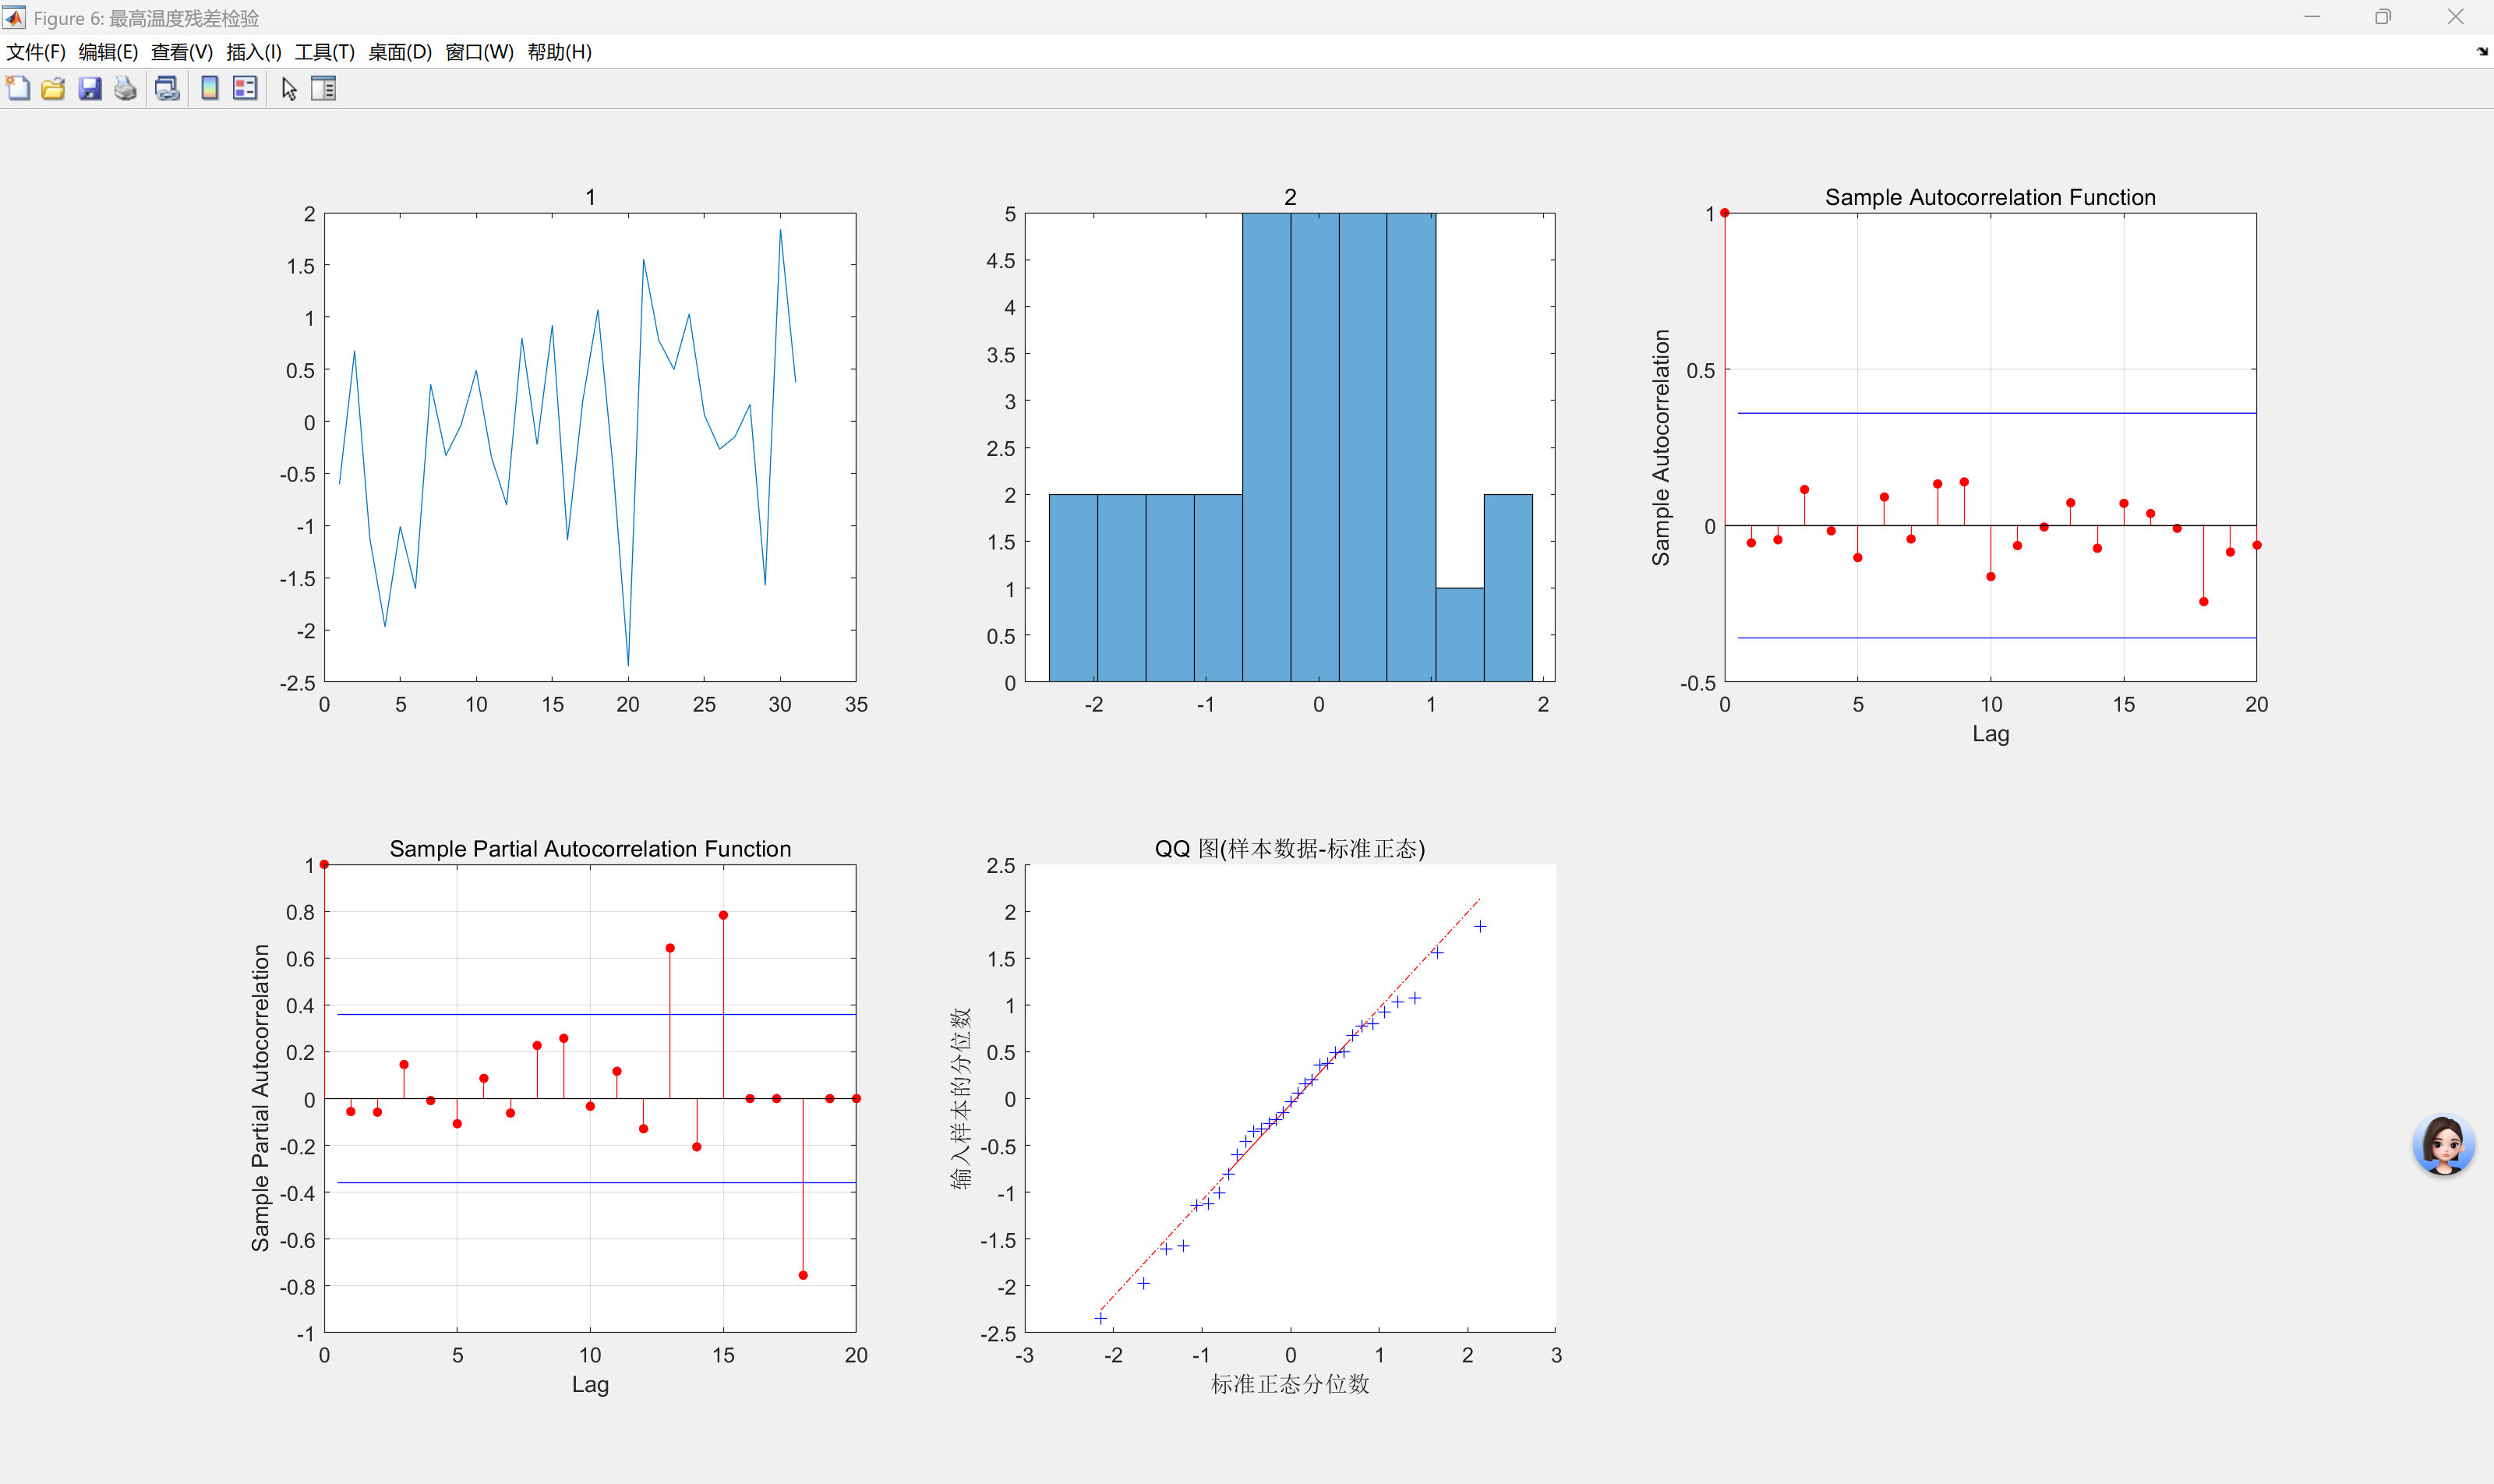
\includegraphics[width=0.45\textwidth]{高温残差检验.png} \quad
    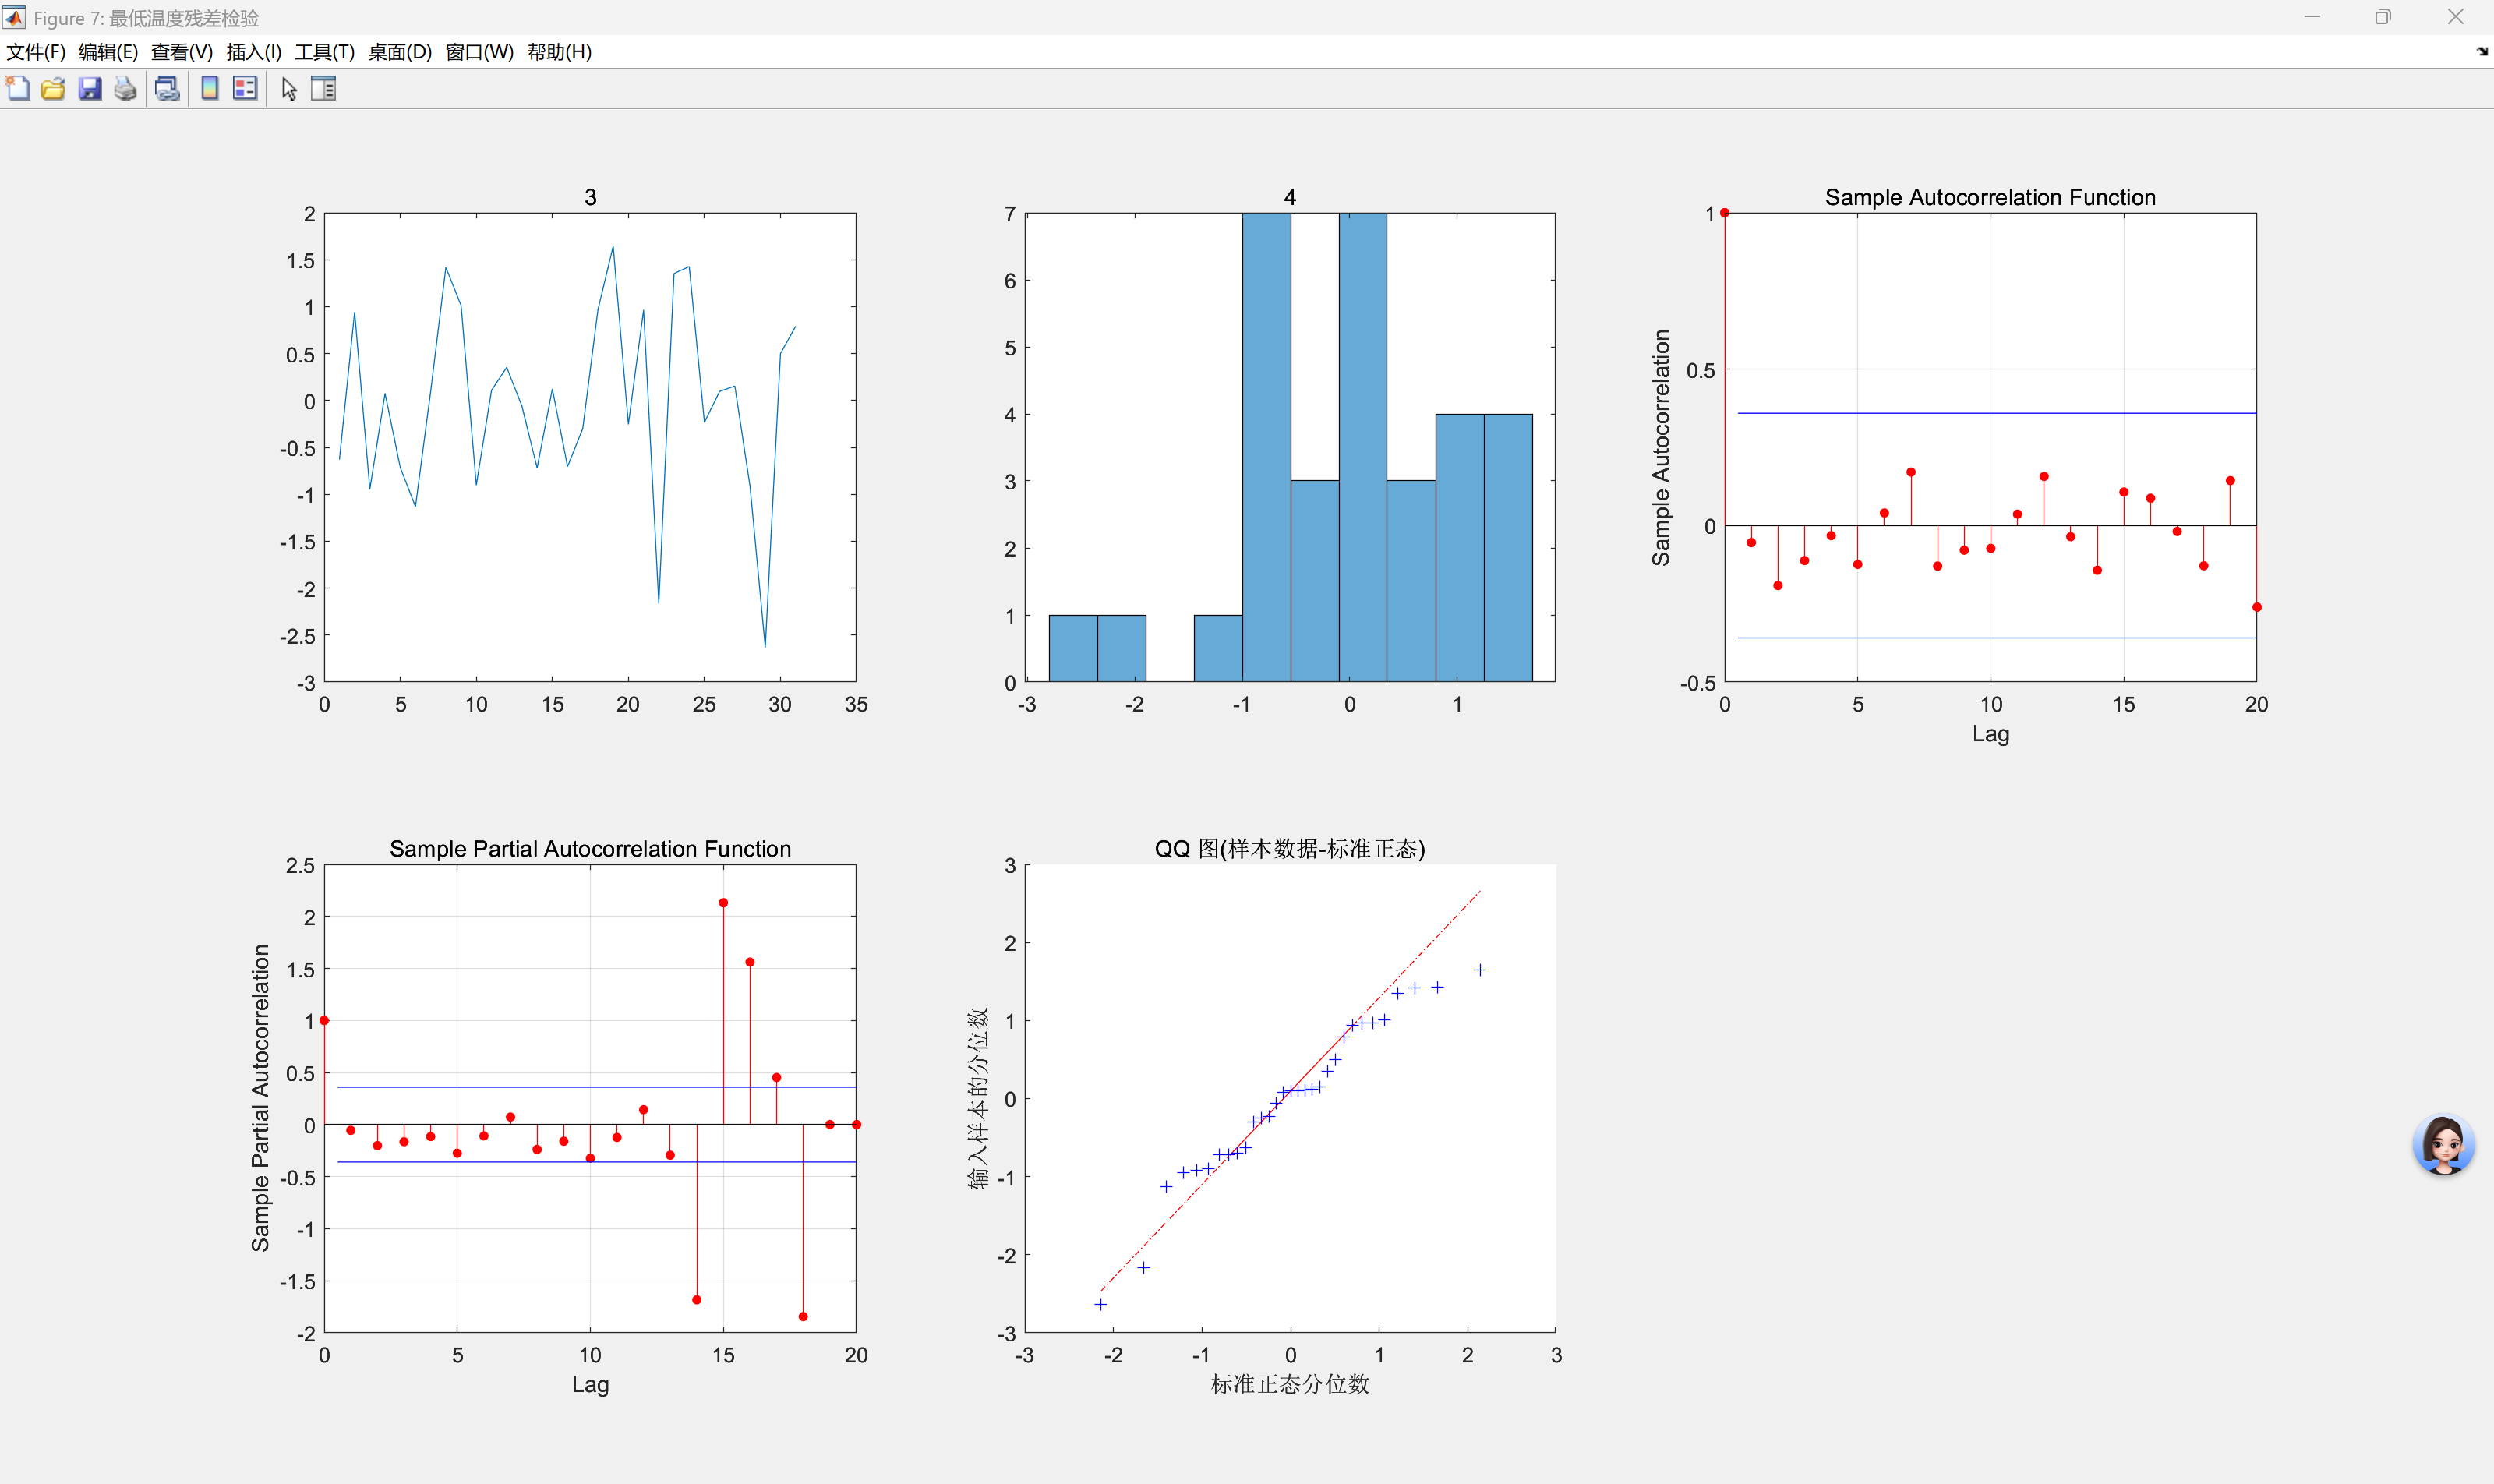
\includegraphics[width=0.45\textwidth]{低温残差检验.png}
    \note{实际汇报时替换为论文中“图6 高温模型残差检验图”和“图7 低温模型残差检验图”}
\end{frame}

\begin{frame}{预测结果展示}
    \begin{block}{9月9日气温预测值}
        \begin{itemize}
            \item 最高气温预测值：31.0982℃（实际值31℃）
            \item 最低气温预测值：13.4087℃（实际值18℃）
        \end{itemize}
    \end{block}
    \centering
    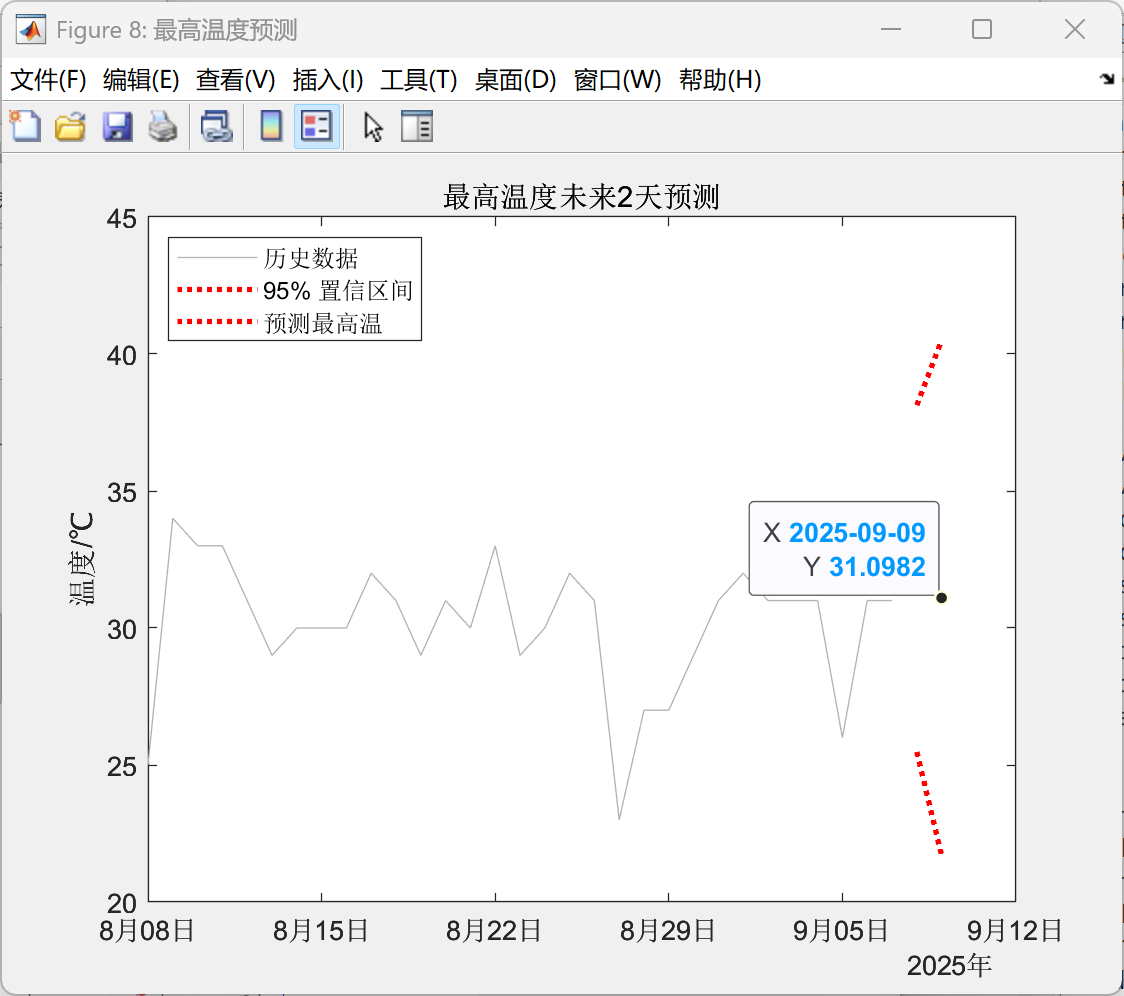
\includegraphics[width=0.48\textwidth]{高温预测.png} \quad
    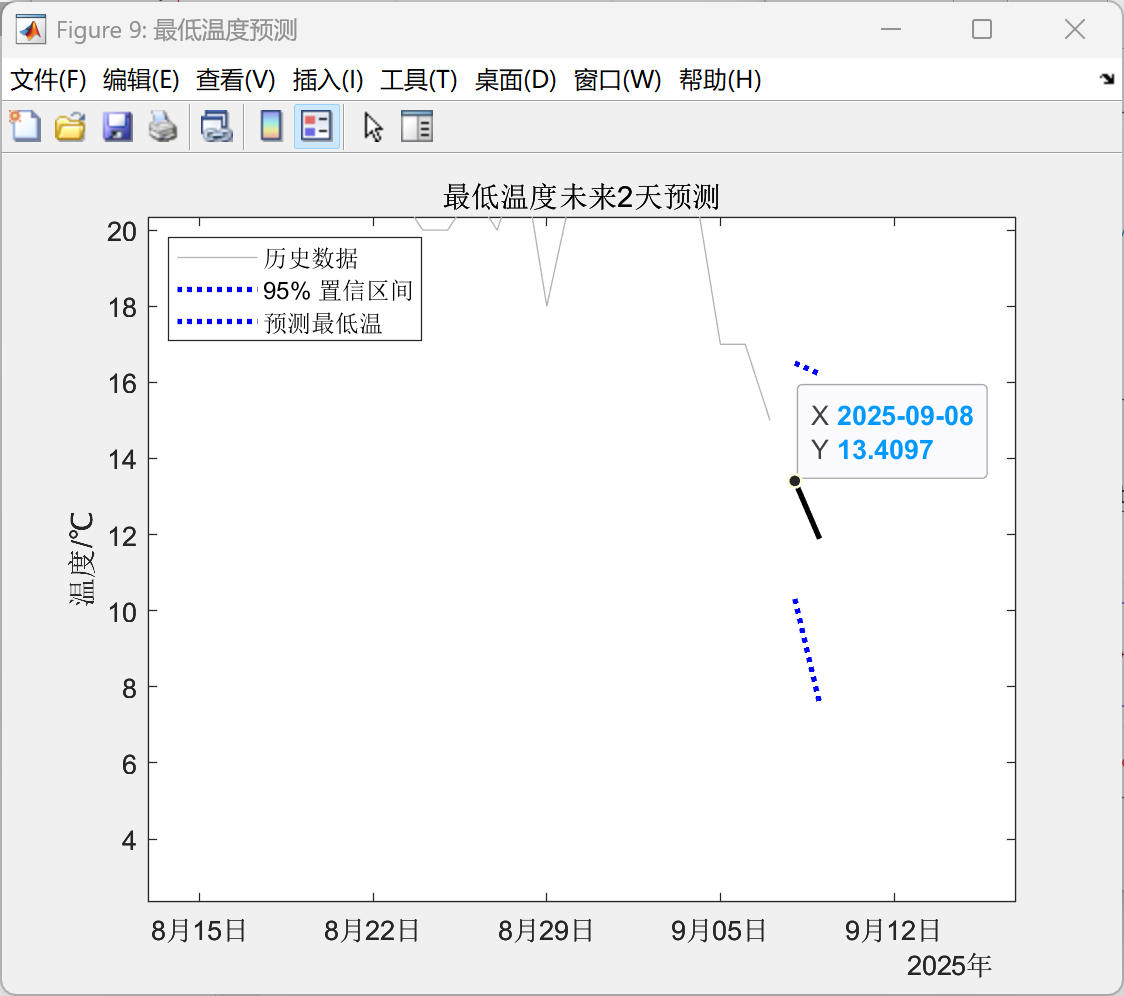
\includegraphics[width=0.48\textwidth]{低温预测.png}
    \note{实际汇报时替换为论文中“图8 高温序列预测图”和“图9 低温序列预测图”}
\end{frame}

% 5.结果分析与讨论
\section{结果分析与讨论}
\begin{frame}{预测精度评估}
    \centering
    \begin{tabular}{|c|c|c|c|c|}
        \hline
        气温类型 & 预测值(℃) & 实际值(℃) & 绝对误差(℃) & 相对误差(\%) \\
        \hline
        最高气温 & 31.0982 & 31 & 0.0982（≈0） & 0.32（≈0） \\
        最低气温 & 13.4087 & 18 & 4.5913（≈5） & 25.51（≈27.8） \\
        \hline
        \multicolumn{3}{|c|}{平均绝对误差（MAE）} & 2.5℃ & - \\
        \multicolumn{3}{|c|}{平均绝对百分比误差（MAPE）} & - & 15.8\% \\
        \hline
    \end{tabular}
    \begin{block}{精度总结}
        最高气温预测精度极高（误差近乎0），最低气温预测存在显著偏差
    \end{block}
\end{frame}

\begin{frame}{误差原因分析}
    \begin{enumerate}
        \item \textbf{数据量不足}：仅32天数据，无法充分捕捉最低气温复杂变化规律（如周期性）
        \item \textbf{模型局限性}：ARIMA为纯时间序列模型，未纳入云量、湿度、风速等外部气象因素
        \item \textbf{微气候影响}：房山区复杂地形导致局部微气候差异，有限数据难以体现
        \item \textbf{极端天气干扰}：9月9日可能存在暖空气突袭、云层保温等未预测的特殊气象条件
    \end{enumerate}
\end{frame}

% 6.结论与展望
\section{结论与展望}
\begin{frame}{研究结论}
    \begin{block}{核心结论}
        \begin{itemize}
            \item 经2阶差分后，房山区8-9月气温序列平稳，适合ARIMA模型建模
            \item ARIMA(1,2,2)（高温）、ARIMA(2,2,0)（低温）模型参数显著，残差为白噪声
            \item 模型短期预测效果良好，最高气温预测精度极高，为有限数据场景提供参考
        \end{itemize}
    \end{block}
    \begin{block}{研究局限性}
        \begin{itemize}
            \item 数据量小（31天），模型泛化能力待验证
            \item 未融合多源气象数据，忽略外部影响因素
            \item 无法捕捉长期气温变化趋势，仅适用于1-7天短期预测
        \end{itemize}
    \end{block}
\end{frame}

\begin{frame}{未来研究方向}
    \begin{enumerate}
        \item \textbf{数据积累}：收集1年以上长时序气温数据，提升模型稳健性
        \item \textbf{多源数据融合}：纳入降水、风速、云量等气象因素，构建多变量预测模型
        \item \textbf{模型改进}：尝试ARIMA与LSTM、随机森林的混合模型，提升非线性拟合能力
        \item \textbf{地形因子嵌入}：结合GIS地形数据，修正局部微气候对气温预测的影响
    \end{enumerate}
    \vspace{2em}
    \centering
    \textbf{感谢聆听！}
\end{frame}